\chapter{Wyniki, testy i analiza skuteczności}
\label{chap:testy-analiza}

\section{Opis przygotowanych testów}

Testy aplikacji \textit{IdentityCore} miały sprawdzić praktyczne działanie dwóch modułów biometrycznych: identyfikacji twarzy oraz identyfikacji odcisku palca. Zależało przede wszystkim na potwierdzeniu, czy system poprawnie zachowuje się w dwóch podstawowych sytuacjach: gdy próbka należy do osoby zapisanej w bazie oraz gdy próbka nie powinna zostać zaakceptowana jako dopasowanie.

Dla obu modalności przygotowano po dwa przypadki testowe. Pierwszy był przypadkiem pozytywnym, w którym oczekiwano znalezienia dopasowania do osoby zarejestrowanej w systemie. Drugi był przypadkiem negatywnym, w którym system powinien zwrócić brak dopasowania. W ten sposób możliwe było sprawdzenie nie tylko samego mechanizmu rozpoznawania, ale również działania progów decyzyjnych, sposobu prezentacji wyniku oraz zgodności zaprezentowanej decyzji z rzeczywistą sytuacją testową.

Próby nie miały charakteru szerokiej walidacji statystycznej. Ich celem było sprawdzenie, czy przygotowany prototyp działa zgodnie z założeniami projektowymi i czy oba moduły biometryczne potrafią zarówno wskazać poprawnego kandydata, jak i odrzucić próbkę niespełniającą warunków akceptacji.

\section{Dane testowe}

Do badań wykorzystano cztery próby: dwie dotyczące twarzy oraz dwie dotyczące odcisku palca. Zestaw został dobrany w sposób prosty, ale celowy: dla każdej modalności uwzględniono jedną próbkę, dla której system powinien znaleźć dopasowanie, oraz jedną próbkę, dla której powinien zwrócić brak dopasowania. Dane testowe zestawiono w tabeli~\ref{tab:dane-testowe}.

\renewcommand{\arraystretch}{1.15}
\begin{xltabular}{\textwidth}{|
    >{\RaggedRight\arraybackslash}p{0.8cm}|
    >{\RaggedRight\arraybackslash}p{1.9cm}|
    >{\RaggedRight\arraybackslash}p{1.9cm}|
    >{\RaggedRight\arraybackslash}p{2.9cm}|
    >{\RaggedRight\arraybackslash}X|}

    \hline
    \textbf{Id} & \textbf{Biometria} & \textbf{Plik / źródło} & \textbf{Osoba oczekiwana} & \textbf{Charakter próbki} \\
    \hline
    \endfirsthead

    T1 & Twarz & kamera & Konrad Fugiel & Próbka twarzy osoby zapisanej w bazie, dla której oczekiwano poprawnego dopasowania. \\
    \hline
    T2 & Twarz & kamera & Brak dopasowania & Próbka twarzy osoby niewystępującej w bazie, przygotowana w celu sprawdzenia poprawnego odrzucenia. \\
    \hline
    O1 & Odcisk palca & plik & Filip Lisowski & Próbka odcisku palca osoby zapisanej w bazie, dla której oczekiwano poprawnego dopasowania. \\
    \hline
    O2 & Odcisk palca & plik & Brak dopasowania & Próbka odcisku palca, dla której system nie powinien znaleźć osoby w bazie. \\
    \hline

    \caption{Zestaw danych testowych wykorzystanych podczas oceny działania systemu}
    \label{tab:dane-testowe}
\end{xltabular}

Przygotowany zestaw jest niewielki, dlatego nie stanowi podstawy do wyznaczania miar statystycznych charakterystycznych dla pełnych badań biometrycznych. Pozwala jednak ocenić, czy system działa poprawnie w podstawowych, kontrolowanych scenariuszach pozytywnych i negatywnych.

\section{Wyniki działania systemu}

Wyniki działania systemu przedstawiono osobno dla identyfikacji twarzy i identyfikacji odcisku palca. Dla obu modułów zestawiono rezultat oczekiwany z rezultatem zwróconym przez aplikację, a następnie pokazano odpowiadające im zrzuty ekranu z wykonanych prób.

\subsection{Wyniki identyfikacji twarzy}

W module identyfikacji twarzy wykonano dwa testy. Pierwszy dotyczył osoby zapisanej w bazie i zakończył się poprawnym dopasowaniem. Drugi test dotyczył osoby niewystępującej w systemie i zakończył się brakiem dopasowania. Zestawienie wyników przedstawiono w tabeli~\ref{tab:wyniki-twarz}.

\renewcommand{\arraystretch}{1.15}
\begin{xltabular}{\textwidth}{|
    >{\RaggedRight\arraybackslash}p{0.8cm}|
    >{\RaggedRight\arraybackslash}p{2.8cm}|
    >{\RaggedRight\arraybackslash}p{3.3cm}|
    >{\RaggedRight\arraybackslash}p{2.2cm}|
    >{\RaggedRight\arraybackslash}X|}

    \hline
    \textbf{Id} & \textbf{Oczekiwany wynik} & \textbf{Wynik systemu} & \textbf{Wynik dopasowania} & \textbf{Ocena} \\
    \hline
    \endfirsthead

    \hline
    \textbf{Id} & \textbf{Oczekiwany wynik} & \textbf{Wynik systemu} & \textbf{Wynik dopasowania} & \textbf{Ocena} \\
    \hline
    \endhead

    T1 & Konrad Fugiel & Znaleziono dopasowanie: Konrad Fugiel & 84,2\% & Poprawne dopasowanie. Wynik przekroczył próg 60,0\%. \\
    \hline
    T2 & Brak dopasowania & Nie znaleziono osoby w bazie & 41,4\% & Brak dopasowania zgodny z oczekiwaniem. Wynik był poniżej progu 60,0\%. \\
    \hline

    \caption{Wyniki testów identyfikacji twarzy}
    \label{tab:wyniki-twarz}
\end{xltabular}

Pierwsza próba twarzy zakończyła się poprawnym rozpoznaniem osoby zapisanej w bazie. System wskazał osobę \textit{Konrad Fugiel}, a wynik podobieństwa osiągnął wartość \(84{,}2\%\). W prawym panelu widoku wynikowego widoczna jest zarówno decyzja \textit{Znaleziono dopasowanie}, jak i szczegóły najlepszego kandydata. Dla tej próby nie pojawił się drugi kandydat, dlatego decyzja została oparta na jednoznacznym najlepszym wyniku.

\begin{figure}[H]
    \centering
    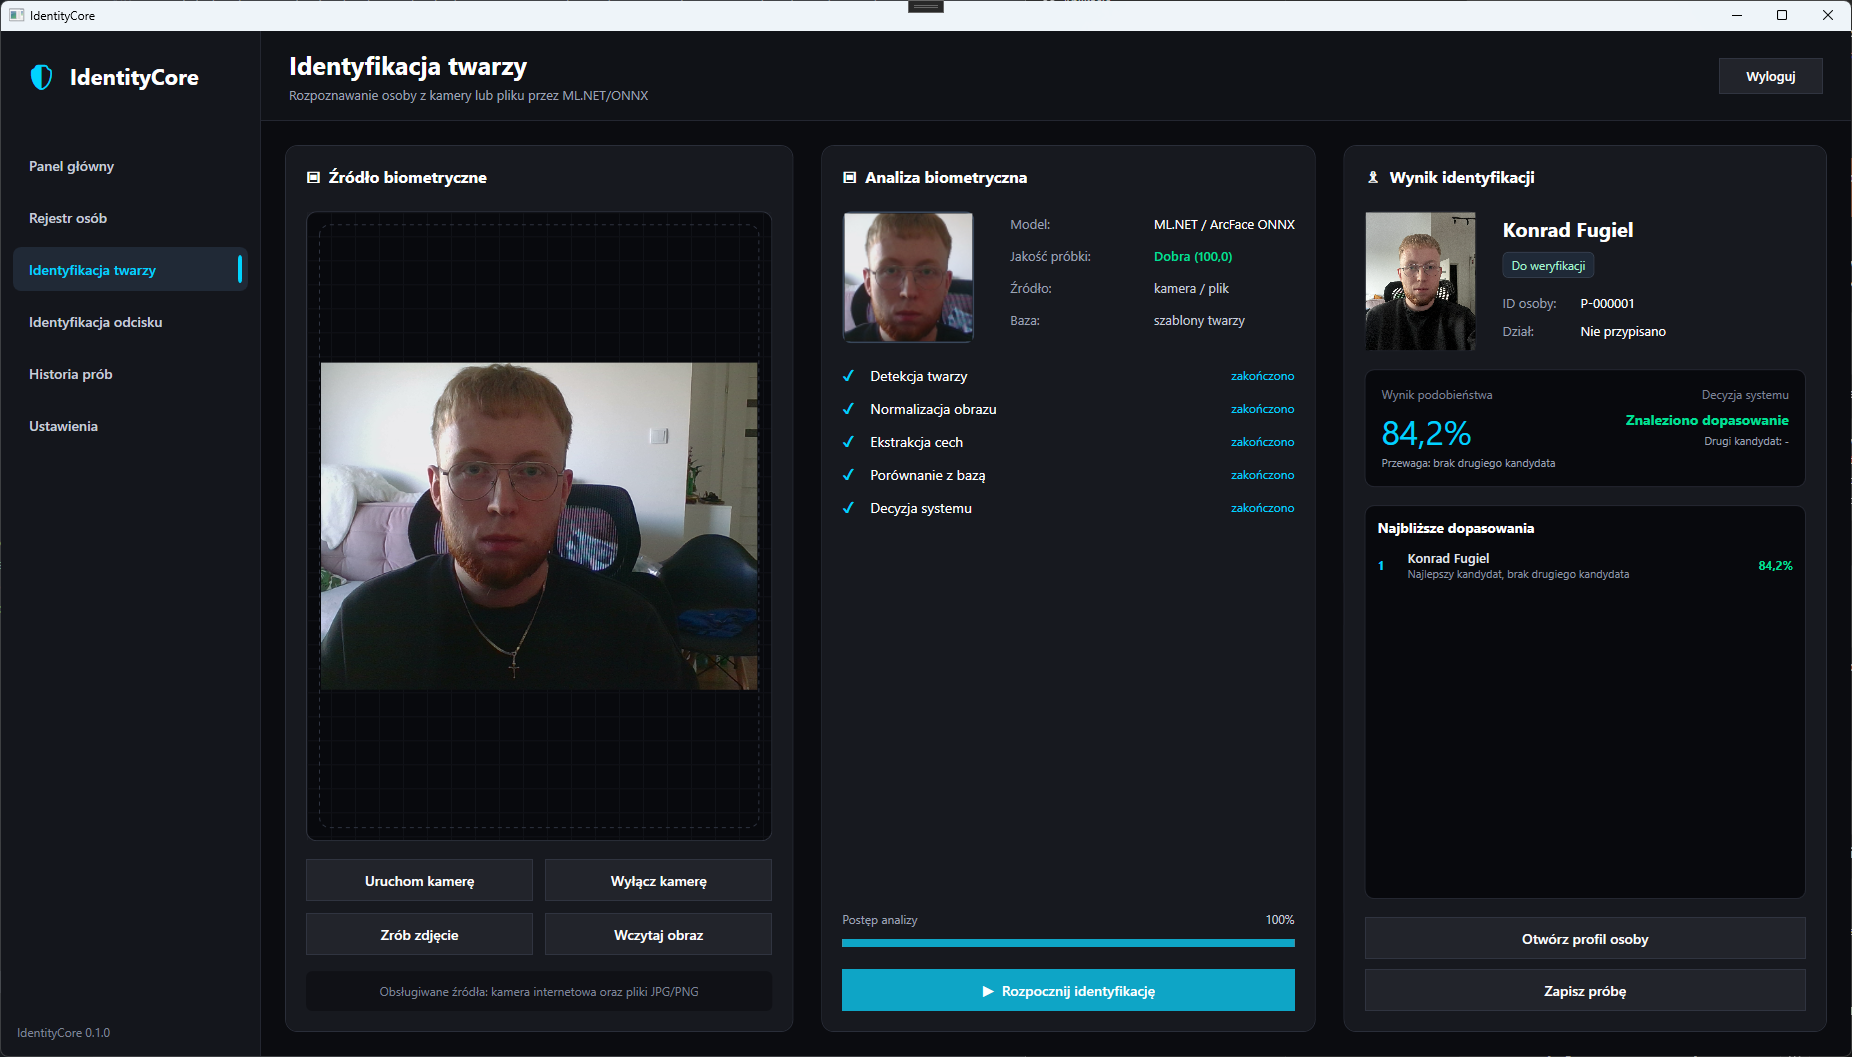
\includegraphics[width=0.98\textwidth]{figures/results/result_01_face_match.png}
    \caption{Wynik pozytywnej identyfikacji twarzy}
    \label{fig:result-face-match}
\end{figure}

Druga próba twarzy miała charakter negatywny. Do systemu wprowadzono twarz osoby niewystępującej w bazie, dlatego oczekiwano odrzucenia wyniku. System rzeczywiście nie zaakceptował dopasowania i zwrócił komunikat \textit{Nie znaleziono osoby w bazie}. Najlepszy uzyskany wynik wyniósł \(41{,}4\%\), co było wartością niższą od ustawionego progu \(60{,}0\%\). W widoku wynikowym pokazano również najbliższe dopasowanie, jednak nie zostało ono zaakceptowane jako rozpoznanie.

\begin{figure}[H]
    \centering
    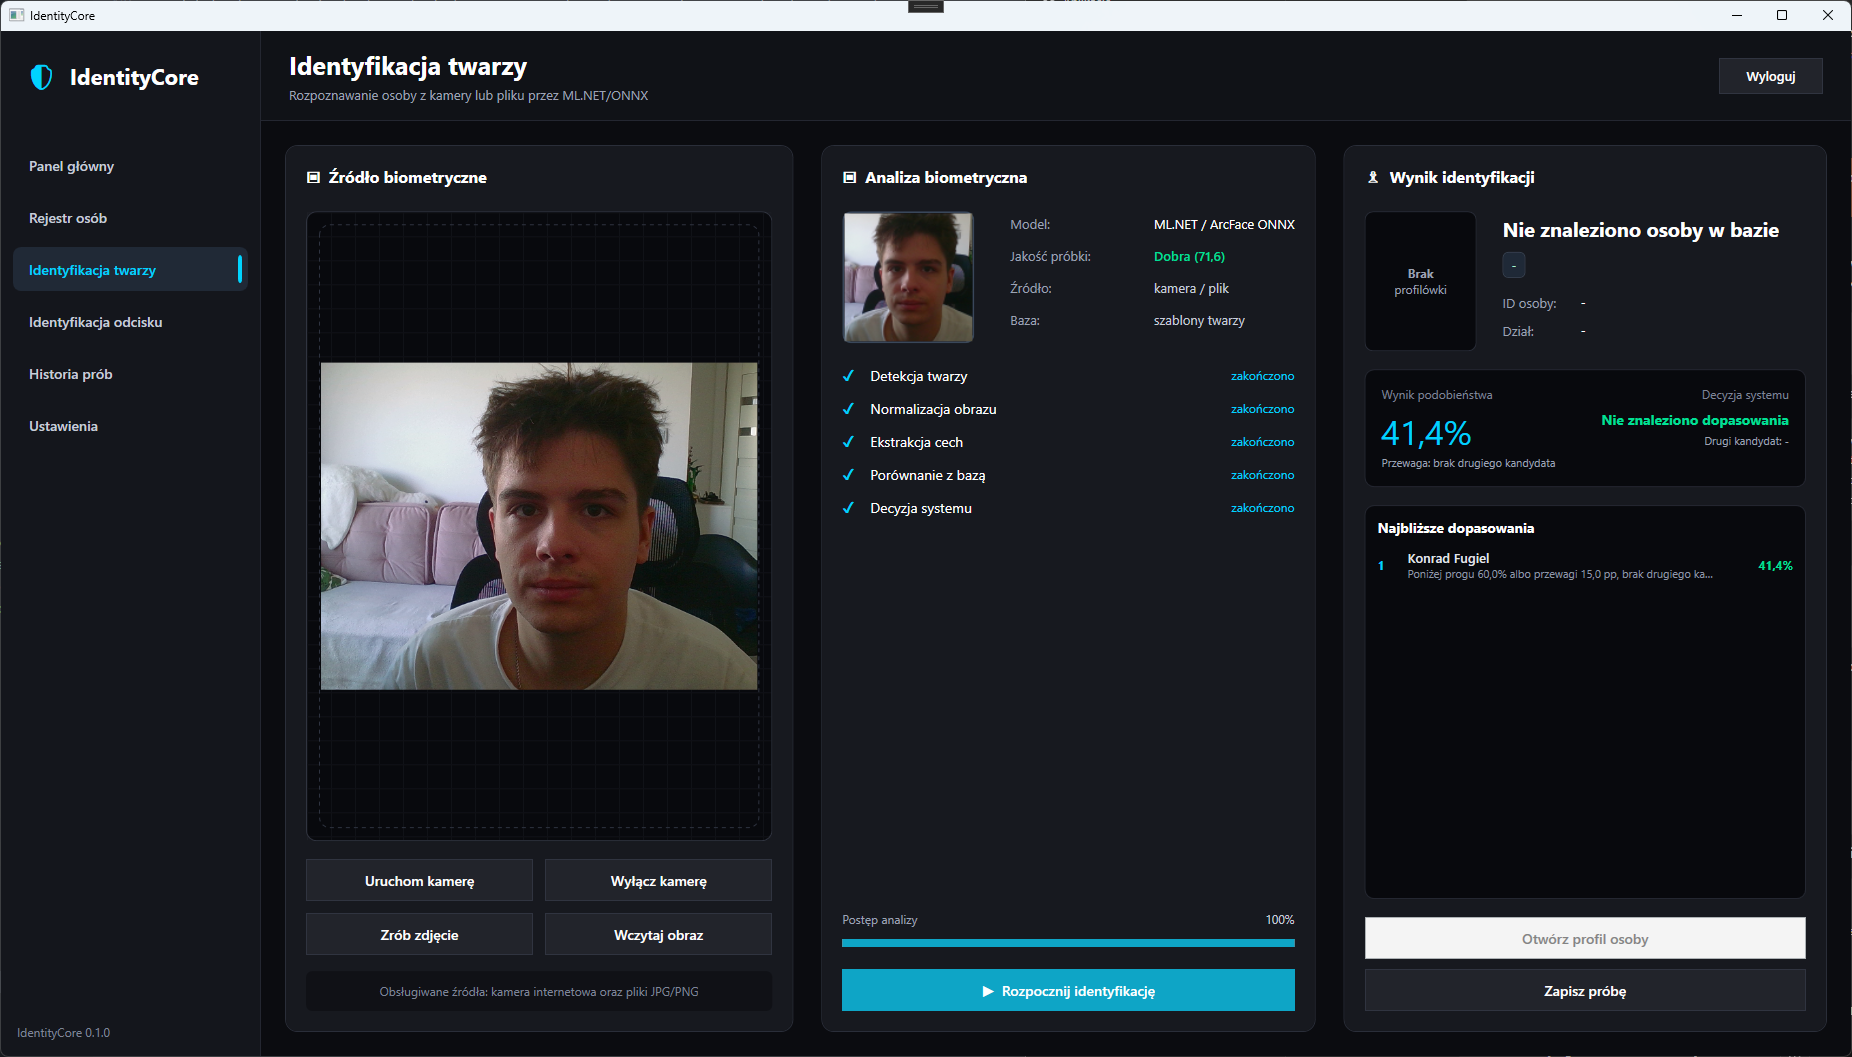
\includegraphics[width=0.98\textwidth]{figures/results/result_02_face_no_match.png}
    \caption{Wynik negatywnej identyfikacji twarzy}
    \label{fig:result-face-no-match}
\end{figure}

\subsection{Wyniki identyfikacji odcisku palca}

W module identyfikacji odcisku palca również przeprowadzono dwa testy: jeden pozytywny oraz jeden negatywny. W pierwszym przypadku system powinien wskazać osobę zapisaną w bazie, a w drugim zwrócić brak dopasowania. Wyniki zestawiono w tabeli~\ref{tab:wyniki-odcisk}.

\renewcommand{\arraystretch}{1.15}
\begin{xltabular}{\textwidth}{|
    >{\RaggedRight\arraybackslash}p{0.8cm}|
    >{\RaggedRight\arraybackslash}p{2.8cm}|
    >{\RaggedRight\arraybackslash}p{3.3cm}|
    >{\RaggedRight\arraybackslash}p{2.2cm}|
    >{\RaggedRight\arraybackslash}X|}

    \hline
    \textbf{Id} & \textbf{Oczekiwany wynik} & \textbf{Wynik systemu} & \textbf{Score dopasowania} & \textbf{Ocena} \\
    \hline
    \endfirsthead

    \hline
    \textbf{Id} & \textbf{Oczekiwany wynik} & \textbf{Wynik systemu} & \textbf{Score dopasowania} & \textbf{Ocena} \\
    \hline
    \endhead

    O1 & Filip Lisowski & Znaleziono dopasowanie: Filip Lisowski & 190,4 & Poprawne dopasowanie. Wynik znacząco przekroczył próg 85,0. \\
    \hline
    O2 & Brak dopasowania & Nie znaleziono osoby w bazie & 9,6 & Brak dopasowania zgodny z oczekiwaniem. Wynik był poniżej progu 85,0. \\
    \hline

    \caption{Wyniki testów identyfikacji odcisku palca}
    \label{tab:wyniki-odcisk}
\end{xltabular}

\newpage

Pozytywna próba odcisku palca została wykonana dla pliku graficznego. System wskazał osobę \textit{Filip Lisowski}, a wynik dopasowania wyniósł \(190{,}4\), czyli wyraźnie przekroczył próg \(85{,}0\). Widok wynikowy pokazuje nie tylko decyzję \textit{Znaleziono dopasowanie}, ale również identyfikator osoby oraz przewagę najlepszego wyniku nad kolejnym kandydatem.

\begin{figure}[H]
    \centering
    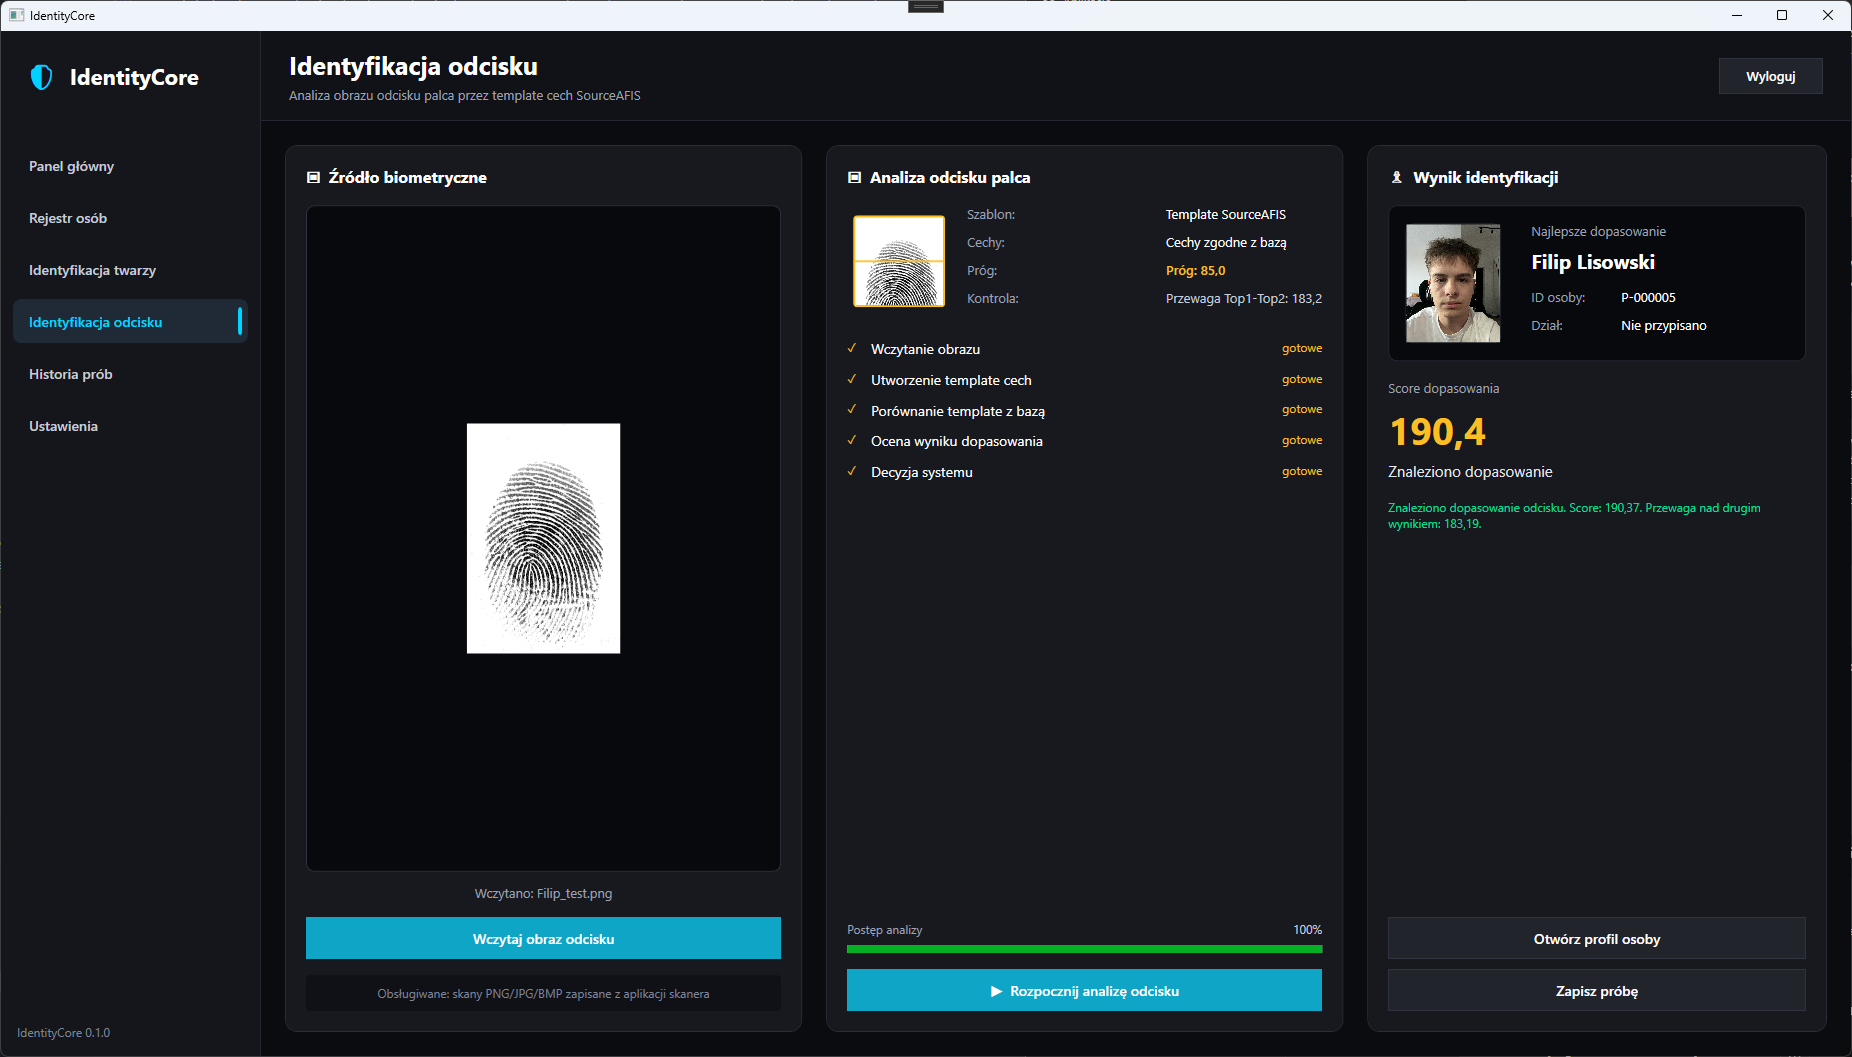
\includegraphics[width=0.98\textwidth]{figures/results/result_03_fingerprint_match.png}
    \caption{Wynik pozytywnej identyfikacji odcisku palca}
    \label{fig:result-fingerprint-match}
\end{figure}

Negatywna próba odcisku palca została wykonana dla pliku \texttt{Konrad\_test\_srodkowy.png}. W tym przypadku system nie znalazł osoby w bazie. Najwyższy uzyskany wynik wyniósł \(9{,}6\), a więc był zdecydowanie niższy od progu \(85{,}0\). Na ekranie widoczna jest również przewaga Top1--Top2 równa \(5{,}7\), jednak już sam bardzo niski wynik dopasowania był wystarczający do odrzucenia próby.

\begin{figure}[H]
    \centering
    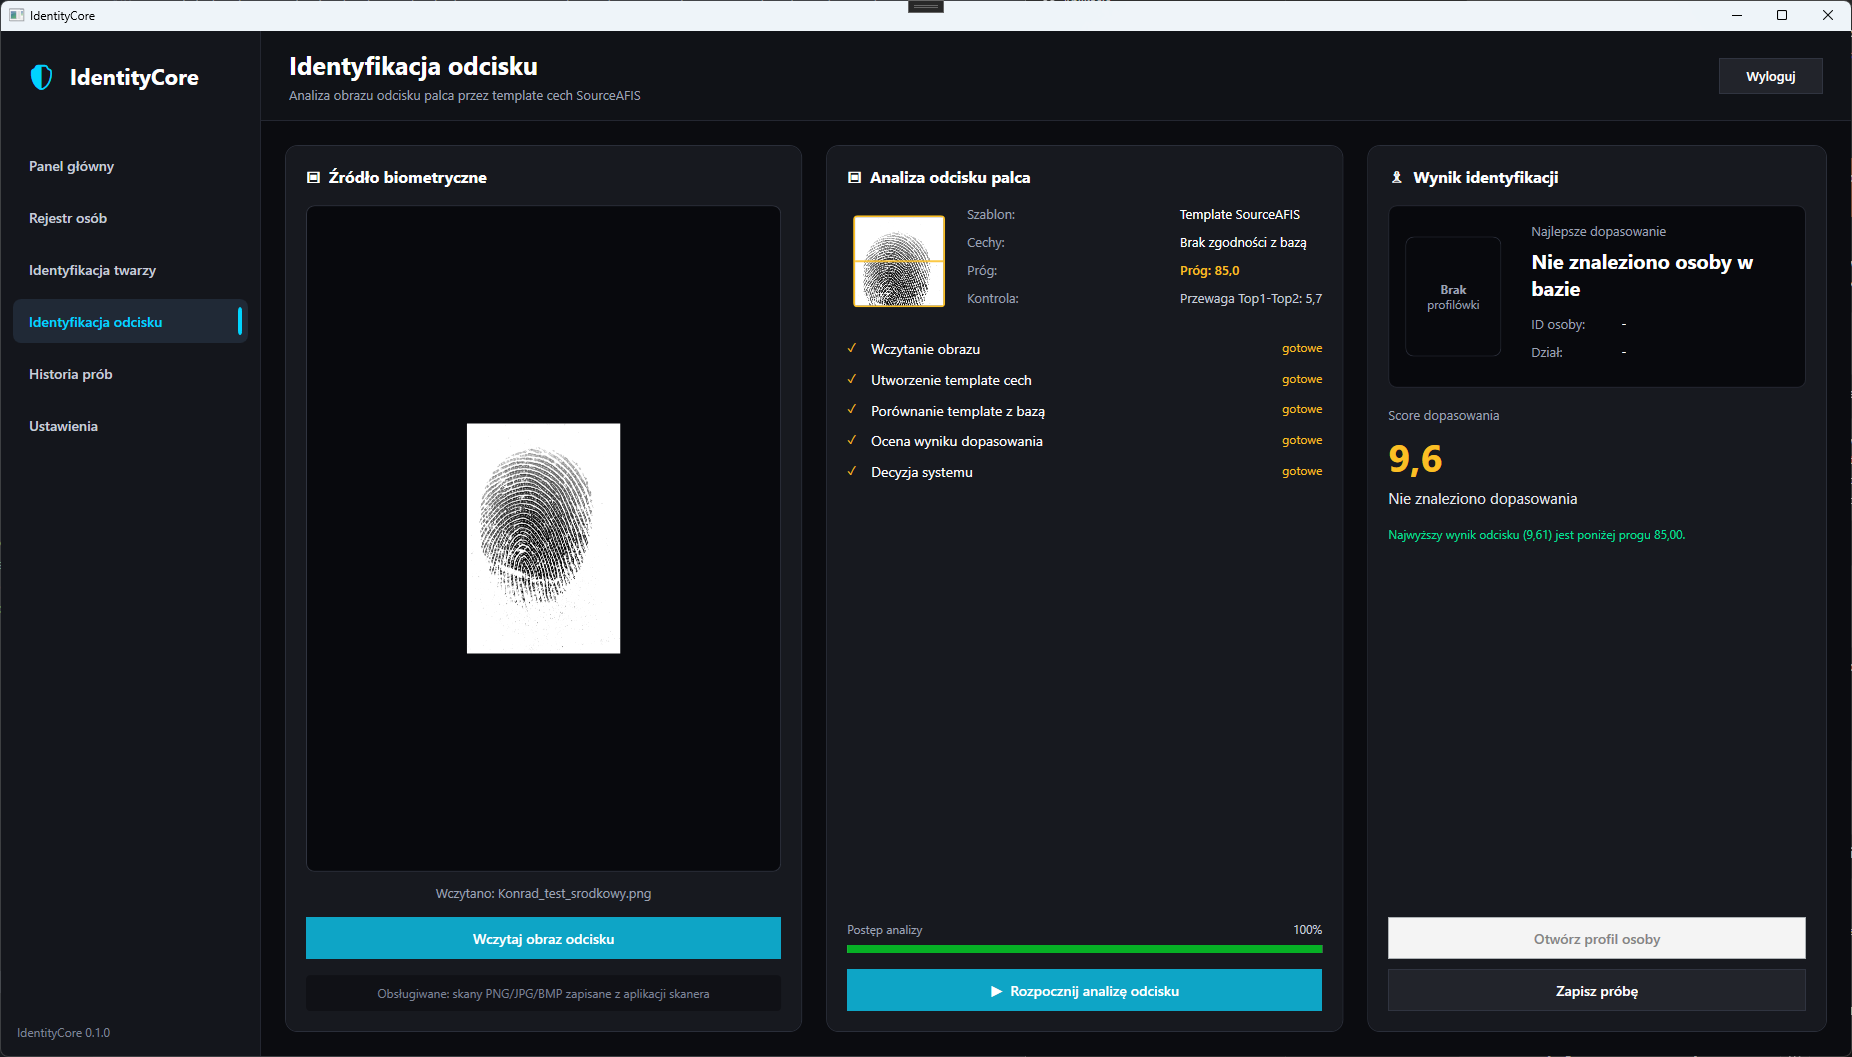
\includegraphics[width=0.98\textwidth]{figures/results/result_04_fingerprint_no_match.png}
    \caption{Wynik negatywnej identyfikacji odcisku palca}
    \label{fig:result-fingerprint-no-match}
\end{figure}

\section{Analiza poprawnych i błędnych rozpoznań}

W przeprowadzonym zestawie testowym wystąpiły zarówno przypadki poprawnego dopasowania, jak i poprawnego braku dopasowania. Dla twarzy system prawidłowo rozpoznał osobę \textit{Konrad Fugiel} przy wyniku \(84{,}2\%\) oraz prawidłowo odrzucił próbkę osoby niewystępującej w bazie przy wyniku \(41{,}4\%\). Dla odcisku palca system poprawnie wskazał osobę \textit{Filip Lisowski} przy wyniku \(190{,}4\) oraz poprawnie odrzucił próbkę negatywną z wynikiem \(9{,}6\).

W badanym zestawie nie wystąpił ani błędny brak dopasowania, ani błędne przypisanie próbki do niewłaściwej osoby. Wystąpiły natomiast dwa przypadki braku dopasowania i w obu sytuacjach był to rezultat zgodny z oczekiwaniem. Oznacza to, że w przygotowanych warunkach testowych system nie tylko znajdował poprawne dopasowania, ale potrafił również odrzucać próbki, które nie powinny zostać zaakceptowane.

Trzeba jednak podkreślić, że wnioski te dotyczą wyłącznie małego zestawu testowego. Wyniki mają charakter poglądowy i pokazują zachowanie prototypu w kilku kontrolowanych przypadkach, a nie pełną ocenę skuteczności systemu biometrycznego.

\section{Wpływ parametrów na działanie systemu}

W aplikacji zastosowano cztery główne parametry decyzyjne: dla twarzy próg podobieństwa \(60{,}0\%\) i margines \(15{,}0\) pp, a dla odcisku palca próg \(85{,}0\) i margines \(15{,}0\). W wykonanych próbach pozytywne przypadki przekroczyły wymagane progi, natomiast obie próby negatywne zostały odrzucone, ponieważ uzyskane wyniki były zbyt niskie.

W praktyce obniżenie progów mogłoby zwiększyć liczbę zaakceptowanych dopasowań, ale jednocześnie podniosłoby ryzyko błędnej akceptacji. Z kolei podwyższenie progów mogłoby poprawić ostrożność decyzji, ale kosztem częstszego odrzucania nawet poprawnych próbek. Dodatkową rolę pełni margines Top1--Top2, który pomaga odrzucać przypadki niejednoznaczne. Zmiana tych ustawień wpływa wyłącznie na kolejne próby i nie modyfikuje wcześniej zapisanych wyników w historii.

\section{Wnioski z eksperymentów}

Przeprowadzone testy potwierdziły, że aplikacja \textit{IdentityCore} realizuje podstawowy cel demonstracyjny. Oba moduły biometryczne potrafiły poprawnie wskazać osobę zapisaną w bazie oraz zwrócić brak dopasowania w sytuacji, gdy próbka nie powinna zostać zaakceptowana.

Najważniejszym ograniczeniem badań jest mała liczba prób. Aby rzetelniej ocenić skuteczność systemu, należałoby przygotować większy i bardziej zróżnicowany zbiór danych, obejmujący więcej osób, więcej przypadków negatywnych oraz próbki o różnej jakości. Na obecnym etapie wyniki należy więc traktować jako potwierdzenie poprawnego działania prototypu, a nie jako pełną walidację skuteczności rozwiązania.